\documentclass[12pt,a4paper]{article}
\usepackage[utf8]{inputenc}
\usepackage[T1]{fontenc}
\usepackage[spanish]{babel}
\usepackage{graphicx}
\usepackage{geometry}
\geometry{margin=1in}
\usepackage{booktabs}
\usepackage{hyperref}
\usepackage{float}

\title{Examen Final: Probabilidad y Estadística para la Inteligencia Artificial}
\author{Martín Brocca \and Agustín López Fredes \and Fermín Rodríguez del Castillo}
\date{Abril 2025}

\begin{document}
\maketitle

\section{Planteamiento del problema}
Don Francisco busca optimizar la gestión de sus supermercados \emph{Santa Ana} y \emph{La Floresta}, respondiendo a:
\begin{enumerate}
  \item \textbf{Vacaciones:} ¿Qué mes presenta las ventas más bajas?  
  \item \textbf{Inversión:} ¿Qué mes presenta las ventas más altas?  
  \item \textbf{Administración de personal:} ¿Cómo varían las ventas según el día de la semana?  
  \item \textbf{Comparación de tiendas:} ¿Existe diferencia significativa entre las medias de ventas?  
\end{enumerate}

\section{Procesamiento de los datos}
Se cargaron los registros diarios (fecha, tienda, monto de ventas) y se procesaron:
\begin{itemize}
  \item Agrupaciones por mes y por día de la semana.  
  \item Cálculo de funciones empíricas de distribución (ECDF) y estimaciones KDE.  
  \item Intervalos de confianza de la media (95\% y 99\%) mediante t-student, ya que las varianzas de la las poblaciones son desconocidas.  
  \item Pruebas de hipótesis: ANOVA y prueba t de una cola.  
\end{itemize}

\section{Resultados}

\subsection{Comparación mensual entre tiendas}
\begin{figure}[H]
  \centering
  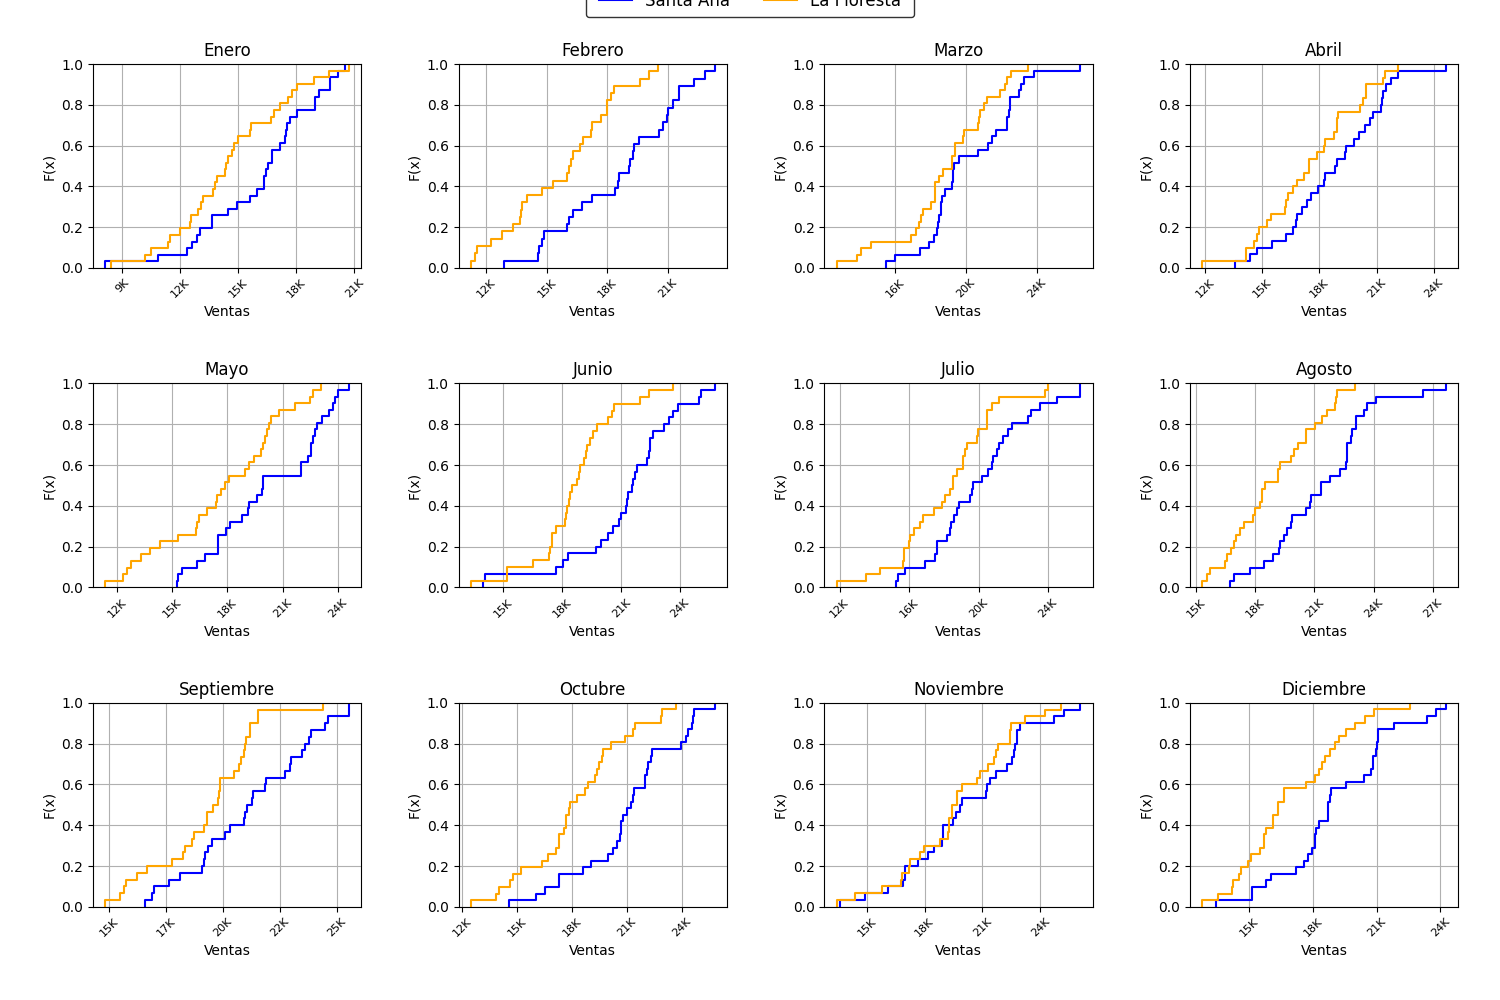
\includegraphics[width=0.8\textwidth]{graphs/SantaAna_vs_LaFloresta_Mensual_ecdf_comparison.png}
  \caption{ECDF de ventas mensuales: Santa Ana vs.\ La Floresta.}
\end{figure}
\begin{figure}[H]
  \centering
  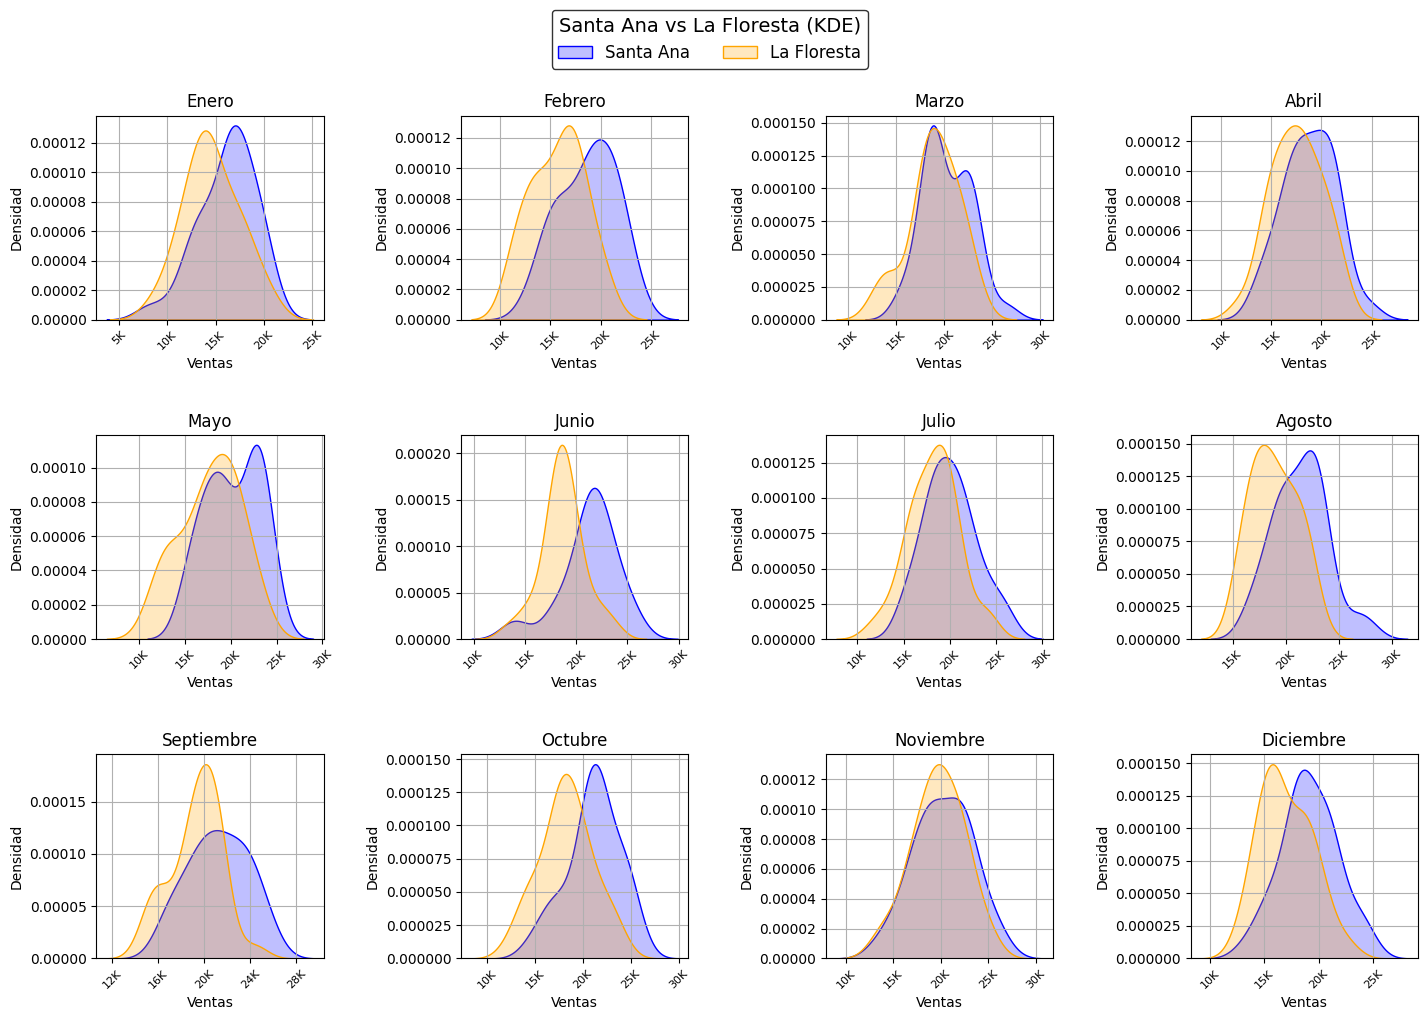
\includegraphics[width=0.8\textwidth]{graphs/SantaAna_vs_LaFloresta_Mensual_kde_comparison.png}
  \caption{Estimación KDE de ventas mensuales: Santa Ana vs.\ La Floresta.}
\end{figure}
\begin{figure}[H]
  \centering
  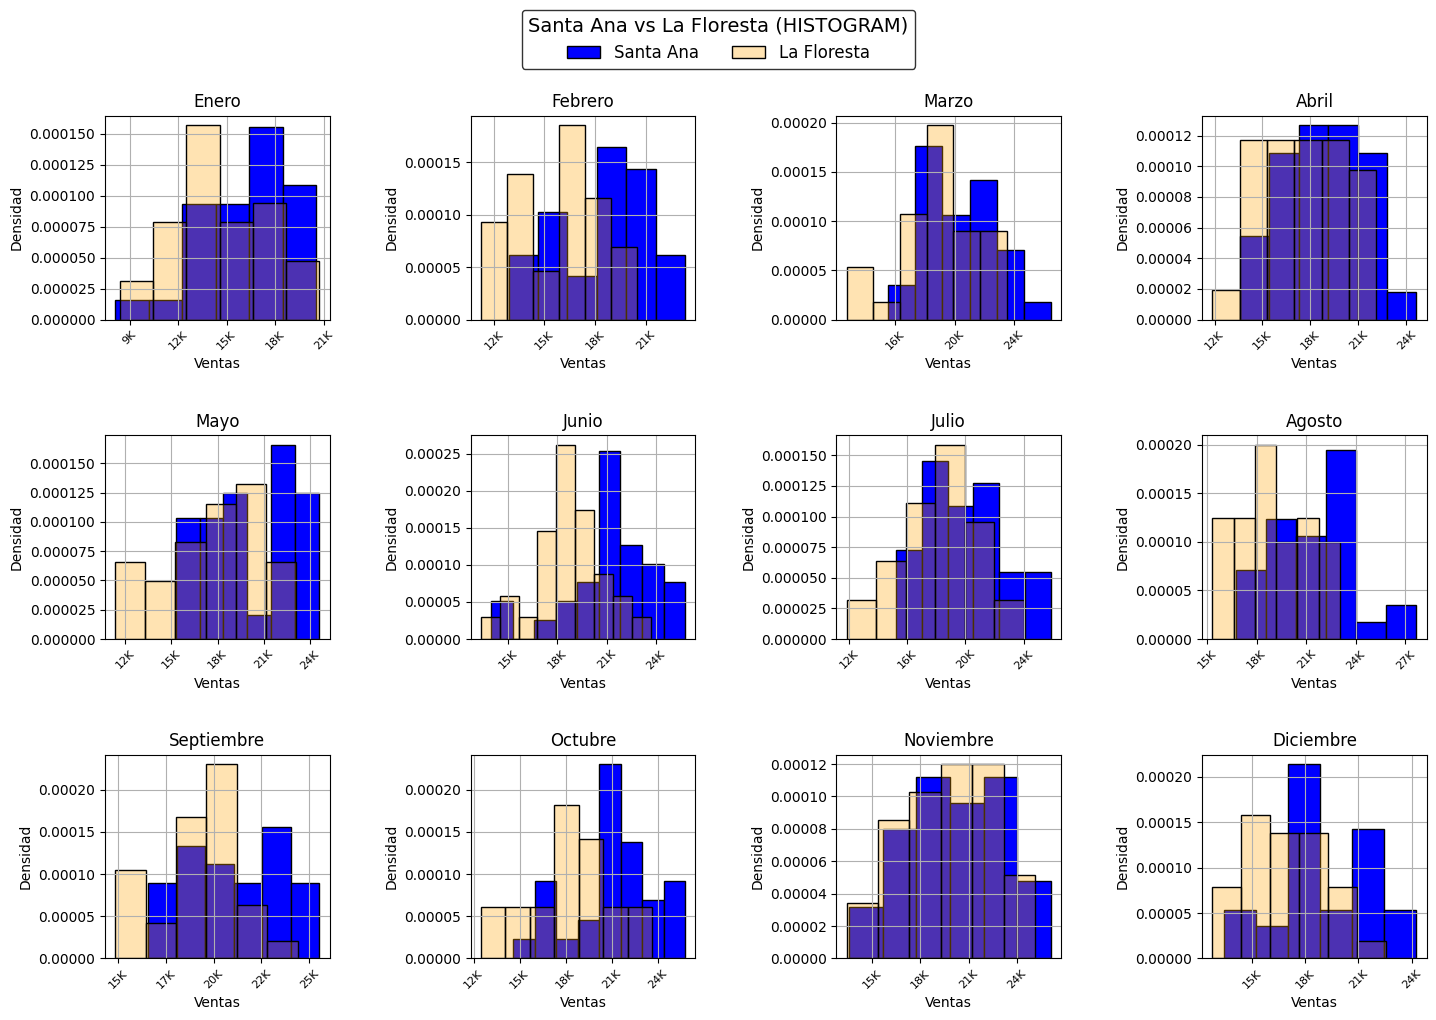
\includegraphics[width=0.8\textwidth]{graphs/SantaAna_vs_LaFloresta_Mensual_histogram_comparison.png}
  \caption{Histograma de ventas mensuales: Santa Ana vs.\ La Floresta.}
\end{figure}

\begin{table}[H]
  \centering
  \small
  \begin{tabular}{c rrrrr | rrrrr}
    \toprule
    Mes & \multicolumn{5}{c}{Santa Ana} & \multicolumn{5}{c}{La Floresta}\\
         & Media & IC95- & IC95+ & IC99- & IC99+ & Media & IC95- & IC95+ & IC99- & IC99+\\
    \midrule
    Ene & 16.1 & 15.0 & 17.2 & 14.7 & 17.6 & 14.8 & 13.7 & 15.9 & 13.2 & 16.3\\
    Feb & 18.6 & 17.5 & 19.8 & 17.2 & 20.1 & 13.9 & 12.8 & 14.9 & 12.5 & 15.3\\
    Mar & 20.3 & 19.4 & 21.2 & 19.1 & 21.5 & 11.5 & 10.3 & 12.7 & 10.0 & 12.9\\
    Abr & 18.8 & 17.8 & 19.7 & 17.5 & 20.1 & 18.9 & 17.8 & 19.9 & 17.6 & 20.2\\
    May & 20.2 & 19.2 & 21.3 & 18.8 & 21.7 & 13.7 & 12.7 & 14.7 & 12.3 & 15.1\\
    Jun & 21.2 & 20.2 & 22.3 & 19.9 & 22.6 & 15.8 & 14.7 & 16.8 & 14.3 & 17.2\\
    Jul & 20.0 & 19.0 & 21.1 & 18.7 & 21.4 & 16.6 & 15.6 & 17.7 & 15.2 & 18.0\\
    Ago & 21.4 & 20.5 & 22.3 & 20.1 & 22.6 & 14.8 & 13.7 & 15.9 & 13.2 & 16.3\\
    Sep & 21.2 & 20.2 & 22.2 & 19.9 & 22.5 & 19.0 & 17.9 & 20.0 & 17.6 & 20.4\\
    Oct & 21.1 & 20.1 & 22.1 & 19.7 & 22.4 & 15.5 & 14.5 & 16.5 & 14.1 & 16.9\\
    Nov & 20.2 & 19.1 & 21.3 & 18.7 & 21.7 & 16.6 & 15.6 & 17.7 & 15.2 & 18.0\\
    Dic & 19.1 & 18.2 & 20.0 & 17.8 & 20.4 & 14.2 & 13.1 & 15.2 & 12.6 & 15.7\\
    \bottomrule
  \end{tabular}
  \caption{IC95\% y IC99\% de la media mensual por tienda (miles)}
\end{table}

\subsection{Ventas mensuales combinadas}
\begin{figure}[H]
  \centering
  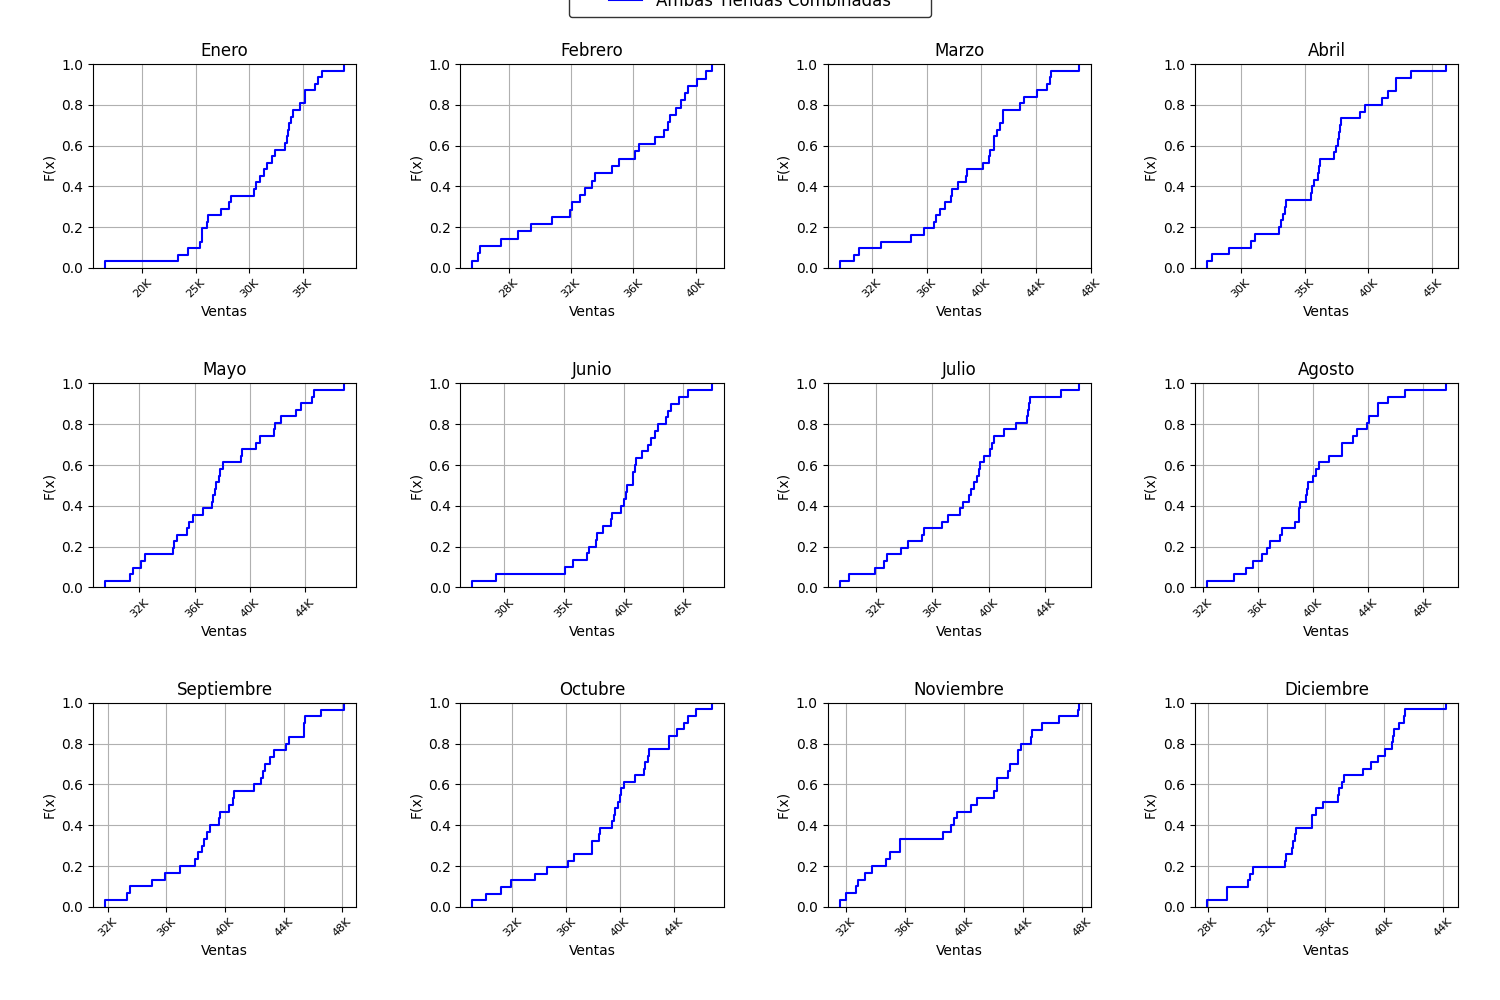
\includegraphics[width=0.8\textwidth]{graphs/Combinado_ecdf_comparison.png}
  \caption{ECDF de ventas mensuales combinadas.}
\end{figure}
\begin{figure}[H]
  \centering
  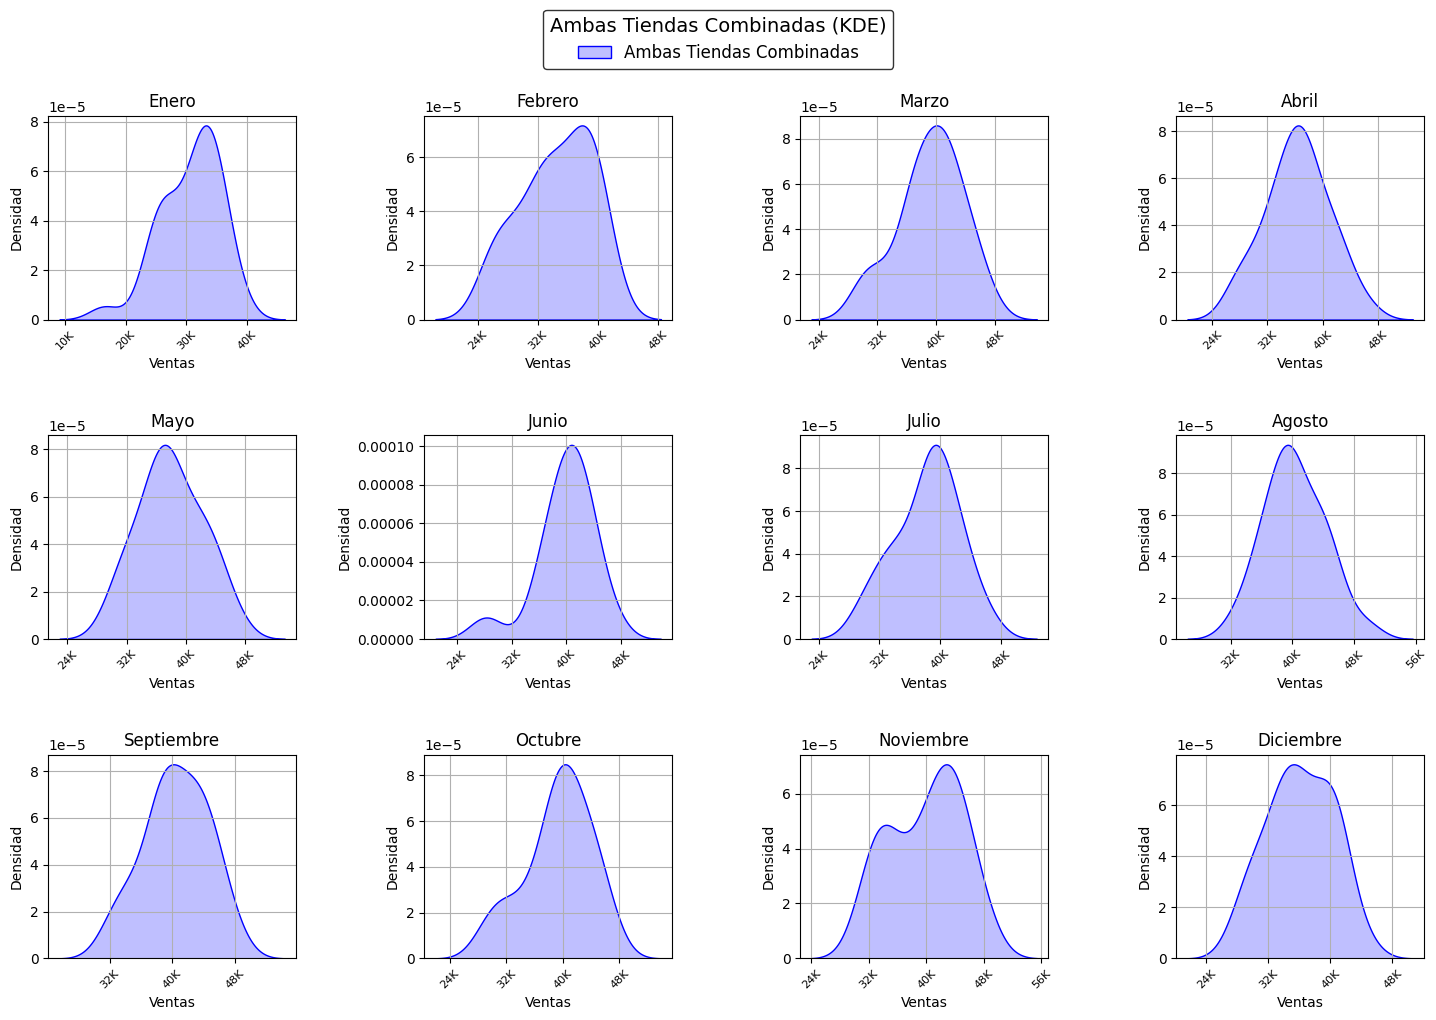
\includegraphics[width=0.8\textwidth]{graphs/Combinado_kde_comparison.png}
  \caption{Estimación KDE de ventas mensuales combinadas.}
\end{figure}
\begin{figure}[H]
  \centering
  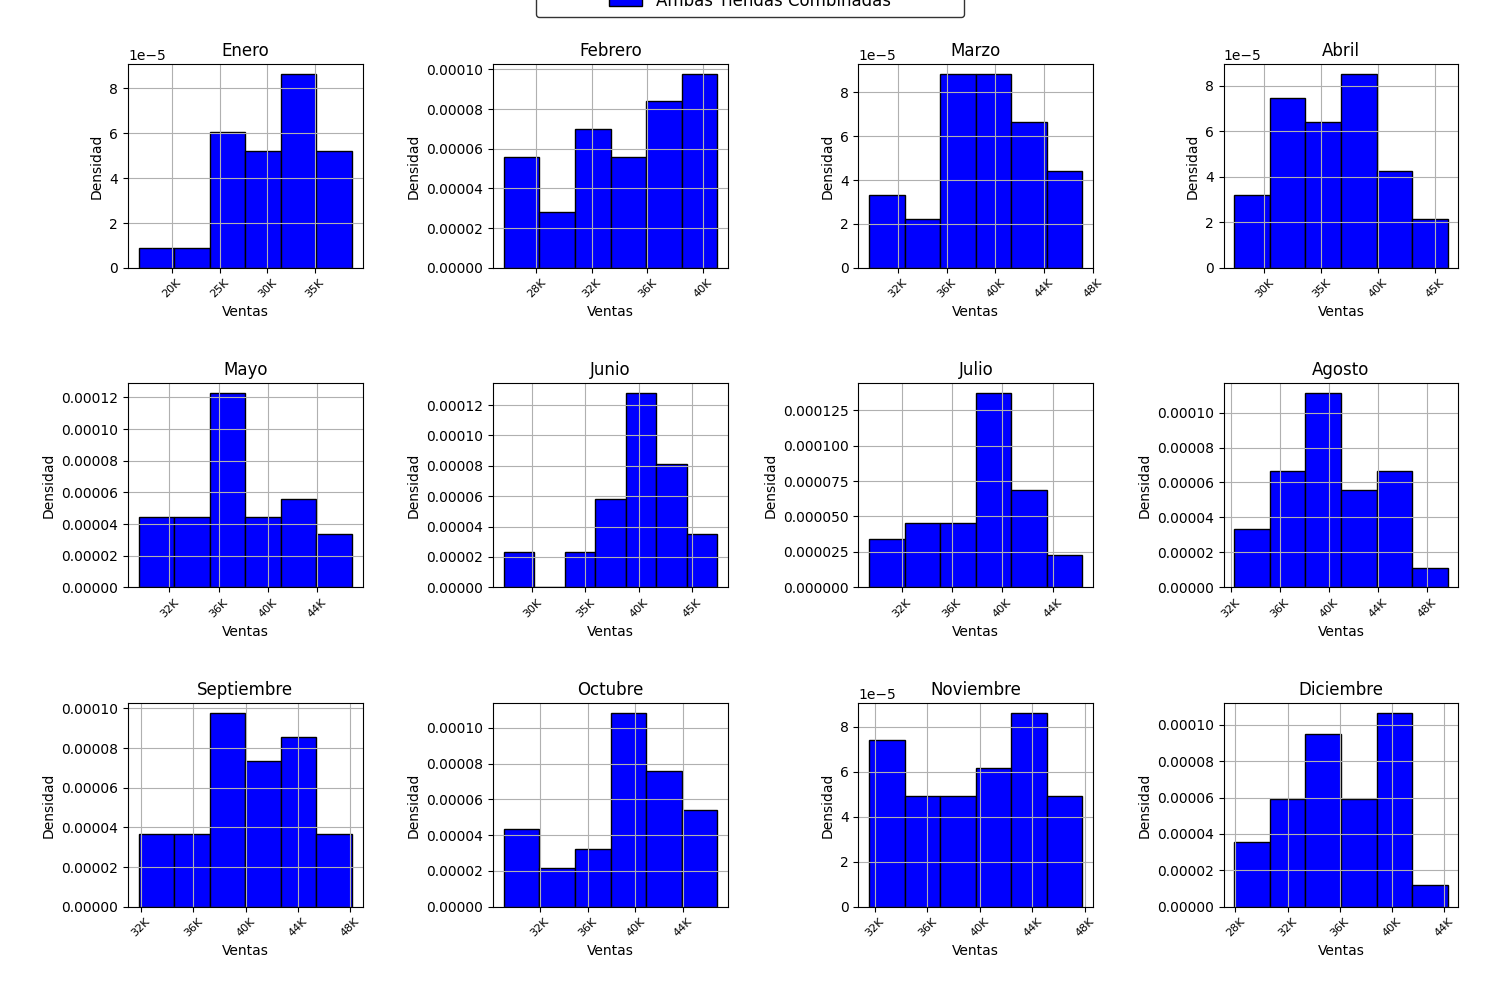
\includegraphics[width=0.8\textwidth]{graphs/Combinado_histogram_comparison.png}
  \caption{Histograma de ventas mensuales combinadas.}
\end{figure}
\begin{table}[H]
  \centering
  \small
  \begin{tabular}{c rrrrr}
    \toprule
    Mes & Media & IC95- & IC95+ & IC99- & IC99+\\
    \midrule
    \textbf{Ene} & 30.9 & 29.0 & 32.8 & 28.4 & 33.4\\
    Feb & 32.5 & 30.6 & 34.4 & 30.0 & 35.0\\
    Mar & 31.8 & 29.9 & 33.7 & 29.3 & 34.3\\
    Abr & 37.7 & 35.6 & 39.8 & 35.0 & 40.4\\
    May & 33.9 & 31.8 & 36.0 & 31.2 & 36.6\\
    Jun & 37.0 & 34.9 & 39.1 & 34.3 & 39.7\\
    Jul & 36.6 & 34.5 & 38.7 & 33.9 & 39.3\\
    Ago & 36.2 & 34.1 & 38.3 & 33.5 & 38.9\\
    \textbf{Sep} & 40.2 & 38.0 & 42.4 & 37.4 & 43.0\\
    Oct & 36.6 & 34.5 & 38.7 & 33.9 & 39.3\\
    Nov & 36.8 & 34.7 & 38.9 & 34.1 & 39.5\\
    Dic & 33.3 & 31.2 & 35.4 & 30.6 & 36.0\\
    \bottomrule
  \end{tabular}
  \caption{IC95\% y IC99\% de la media mensual combinada (miles). Meses clave en negrita.}
\end{table}

\subsection{Comparación diaria entre tiendas}
\begin{figure}[H]
  \centering
  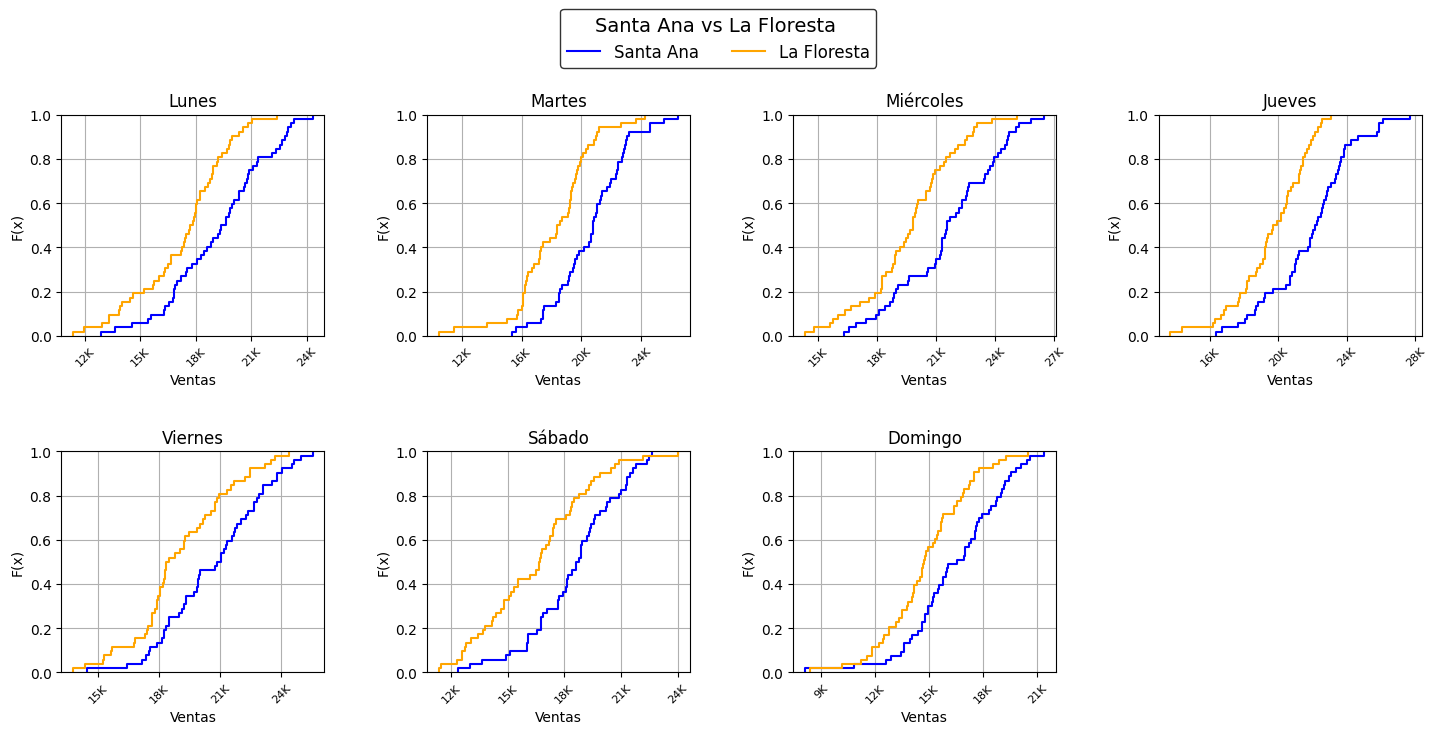
\includegraphics[width=0.8\textwidth]{graphs/SantaAna_vs_LaFloresta_Diario_ecdf_comparison.png}
  \caption{ECDF de ventas diarias: Santa Ana vs.\ La Floresta.}
\end{figure}
\begin{figure}[H]
  \centering
  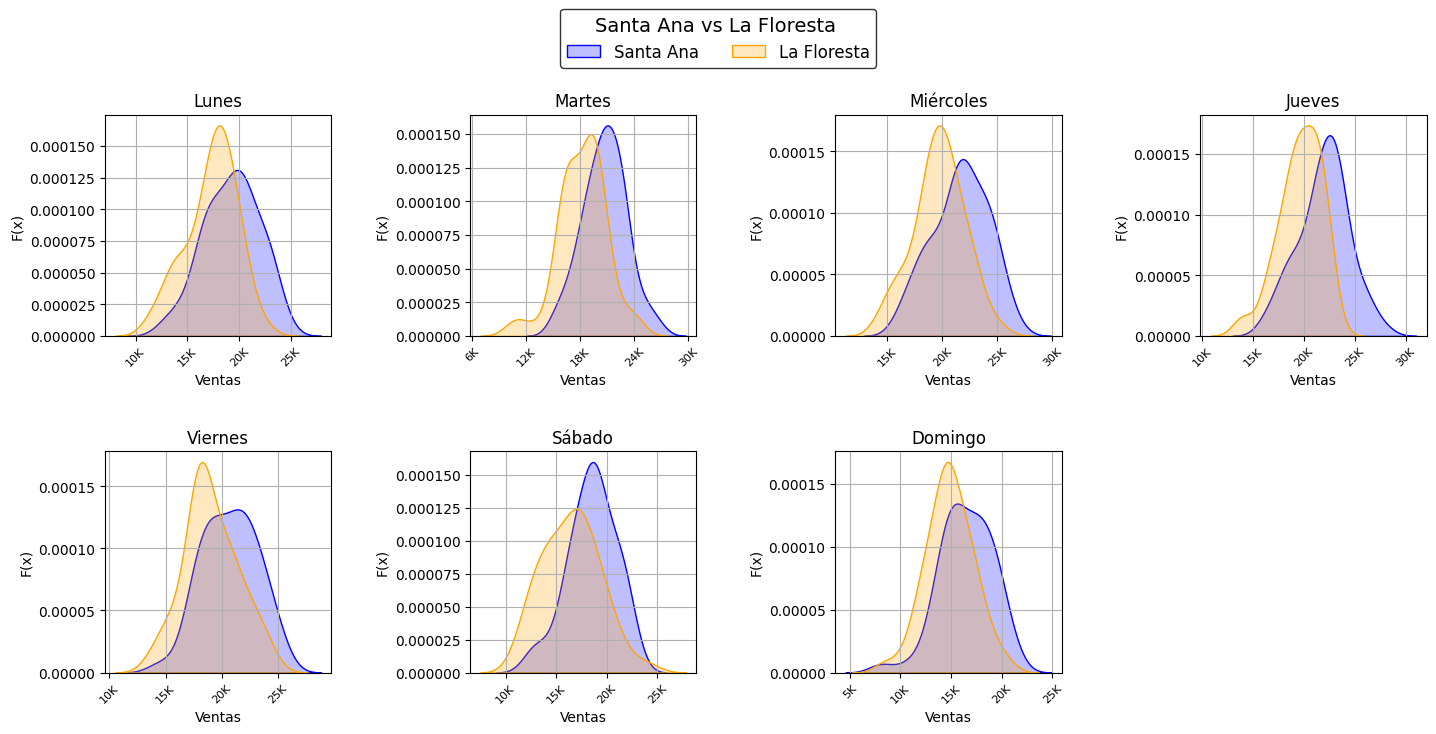
\includegraphics[width=0.8\textwidth]{graphs/SantaAna_vs_LaFloresta_Diario_kde_comparison.png}
  \caption{Estimación KDE de ventas diarias: Santa Ana vs.\ La Floresta.}
\end{figure}
\begin{figure}[H]
  \centering
  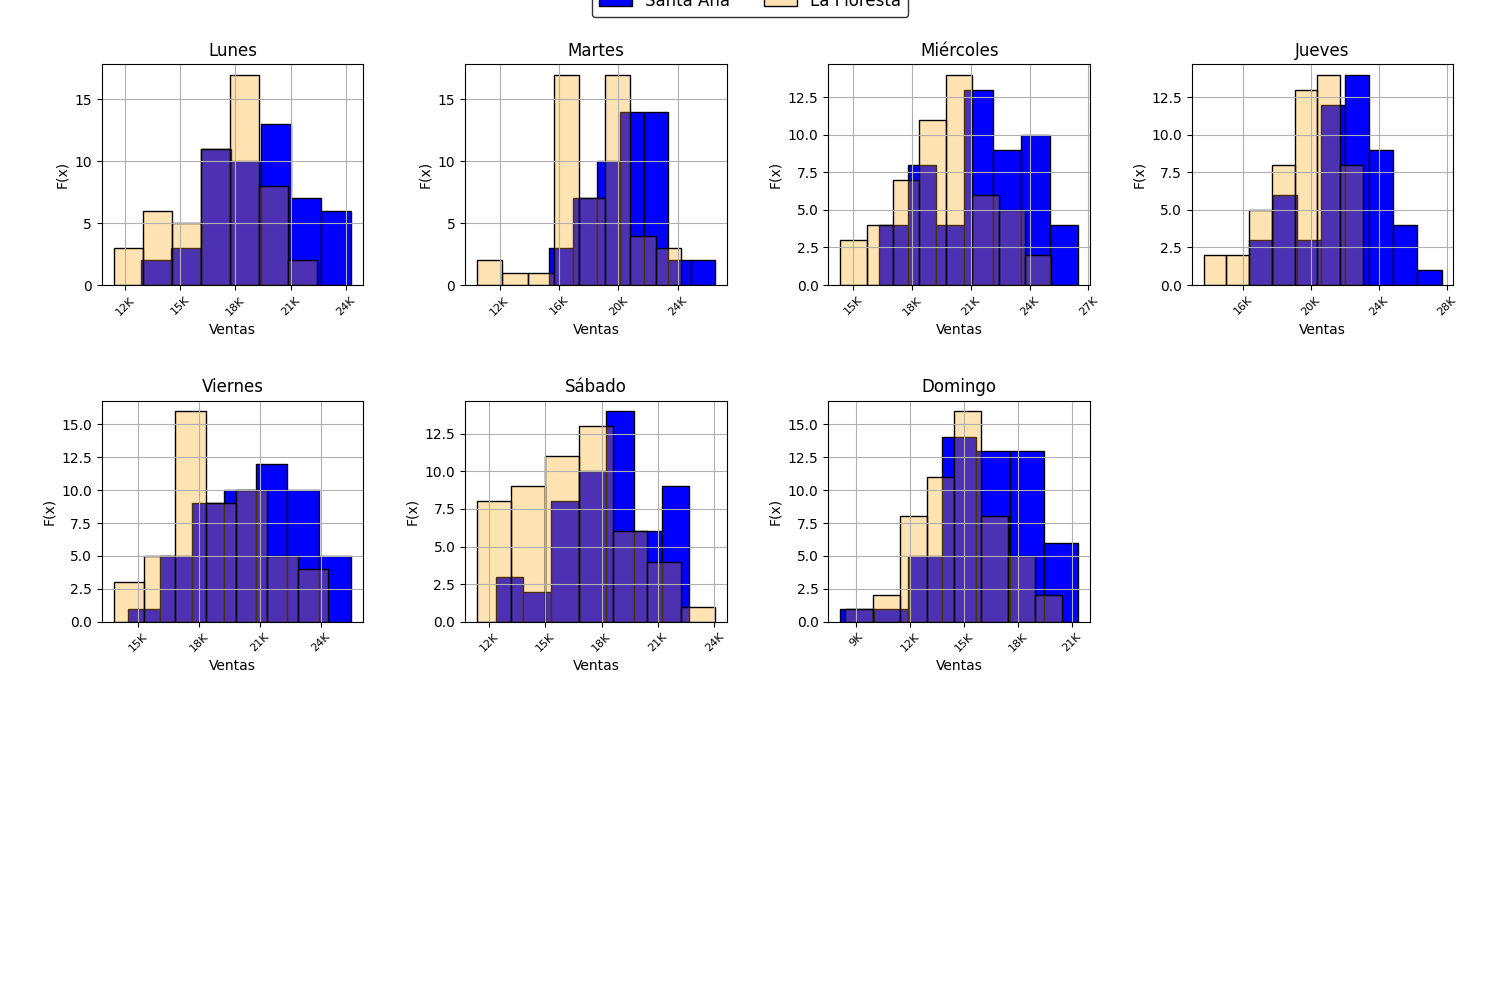
\includegraphics[width=0.8\textwidth]{graphs/SantaAna_vs_LaFloresta_Diario_histogram_comparison.png}
  \caption{Histograma de ventas diarias: Santa Ana vs.\ La Floresta.}
\end{figure}

\begin{table}[H]
  \centering
  \small
  \begin{tabular}{l rrrrr | rrrrr}
    \toprule
    Día & \multicolumn{5}{c}{Santa Ana} & \multicolumn{5}{c}{La Floresta}\\
         & Media & IC95- & IC95+ & IC99- & IC99+ & Media & IC95- & IC95+ & IC99- & IC99+\\
    \midrule
    Lunes     & 19.2 & 18.5 & 20.0 & 18.3 & 20.2 & 17.3 & 16.6 & 18.0 & 16.4 & 18.2\\
    Martes    & 20.7 & 20.0 & 21.3 & 19.8 & 21.5 & 18.2 & 17.5 & 18.9 & 17.2 & 19.2\\
    \textbf{Miércoles} & 21.6 & 20.9 & 22.3 & 20.7 & 22.5 & 19.7 & 19.0 & 20.3 & 18.8 & 20.5\\
    \textbf{Jueves}    & 21.9 & 21.2 & 22.6 & 21.0 & 22.8 & 19.6 & 19.1 & 20.2 & 18.9 & 20.4\\
    Viernes   & 20.7 & 20.0 & 21.4 & 19.8 & 21.6 & 19.0 & 18.4 & 19.7 & 18.2 & 19.9\\
    Sábado    & 18.5 & 17.8 & 19.2 & 17.6 & 19.4 & 16.5 & 15.7 & 17.3 & 15.4 & 17.5\\
    \textbf{Domingo}   & 16.5 & 15.7 & 17.2 & 15.5 & 17.4 & 14.8 & 14.2 & 15.5 & 14.0 & 15.7\\
    \bottomrule
  \end{tabular}
  \caption{IC95\% y IC99\% de la media diaria por tienda (miles). Días clave en negrita.}
\end{table}

\section{Análisis y conclusiones}
En base a los resultados y a los intervalos de confianza, podemos concluir lo siguiente:

\begin{itemize}
  \item En \textbf{enero} la venta promedio combinada fue de 30.9 mil, con intervalo de confianza 95 \% de 29.0 a 32.8 y 99 \% de 28.4 a 33.4, lo que confirma estadísticamente que es el mes de menor actividad y por tanto el más adecuado para tomar vacaciones.
  \item En \textbf{septiembre} se alcanzó el pico máximo combinado, con promedio de 40.2 mil, IC95 \% entre 38.0 y 42.4 e IC99 \% entre 37.4 y 43.0, reflejando que justifica concentrar inversiones en ese mes.
  \item Para ambas tiendas los \textbf{miércoles} y \textbf{jueves} registraron los promedios diarios más altos (21.6 y 21.9 mil): sus IC95\% (20.9–22.3 y 21.2–22.6) e IC99\% (20.7–22.5 y 21.0–22.8) superan la media semanal, por lo que conviene contratar más empleados esos días; en cambio los \textbf{domingos} (16.5 mil, IC95\% 15.7–17.2 y IC99\% 15.5–17.4) presentan la menor demanda y permiten reducir personal.
  \item Santa Ana promedió 19.2 mil al día frente a los 17.3 mil de La Floresta; sus IC95\% (18.5–20.0 vs.\ 16.6–18.0) e IC99\% (18.3–20.2 vs.\ 16.4–18.2) confirman al 95\% y al 99\% la diferencia significativa, demostrando que efectivamente Don Francisco tenía razón y Santa Ana vende más.
\end{itemize}

\section*{Código}
El Notebook completo está en:\newline
\url{https://github.com/martinbrocca/CEIA-PEIA/blob/main/TP3/TP3.ipynb}

\end{document}
